\documentclass[12pt, psamsfonts]{amsart}

%-------Packages---------
\usepackage{amssymb,amsfonts}
\usepackage{todonotes}
\usepackage{fullpage}
\usepackage{physics}
\usepackage[all,arc]{xy}
\usepackage{enumerate}
\usepackage{mathrsfs}
\usepackage{theoremref}
\usepackage{graphicx}
\usepackage[bookmarks]{hyperref}

%--------Theorem Environments--------
%theoremstyle{plain} --- default
\newtheorem{thm}{Theorem}[section]
\newtheorem{cor}[thm]{Corollary}
\newtheorem{prop}[thm]{Proposition}
\newtheorem{lem}[thm]{Lemma}
\newtheorem{conj}[thm]{Conjecture}
\newtheorem{quest}[thm]{Question}

\theoremstyle{definition}
\newtheorem{defn}[thm]{Definition}
\newtheorem{defns}[thm]{Definitions}
\newtheorem{con}[thm]{Construction}
\newtheorem{exmp}[thm]{Example}
\newtheorem{exmps}[thm]{Examples}
\newtheorem{notn}[thm]{Notation}
\newtheorem{notns}[thm]{Notations}
\newtheorem{addm}[thm]{Addendum}
\newtheorem*{exer}{Exercise}

\theoremstyle{remark}
\newtheorem{rem}[thm]{Remark}
\newtheorem{rems}[thm]{Remarks}
\newtheorem{warn}[thm]{Warning}
\newtheorem{sch}[thm]{Scholium}

\DeclareMathOperator{\Hom}{Hom}
\DeclareMathOperator{\Id}{Id}

\makeatletter
\let\c@equation\c@thm
\makeatother
\numberwithin{equation}{section}

\bibliographystyle{plain}

\begin{document}

\title{Math 601 Homework (Due 9/18)}
\author{Hidenori Shinohara}
\maketitle

\begin{exer}{(Problem 1)}
  Let $R$ be a commutative ring with one.
  Explain why there is a unique ring homomorphism, $\mathbb{Z} \rightarrow R$.
\end{exer}

\begin{proof}
  The existence of a ring homomorphism is clear since $\phi(n) = 1_R + \cdots + 1_R$ and $\phi(-n) = -\phi(n)$ define a homomorphism.

  We will show the uniqueness of a ring homomorphism.
  Let $\phi_1, \phi_2: \mathbb{Z} \rightarrow R$ be ring homomorphisms.

  We claim that $\phi_1(n) = \phi_2(n)$ for each $n \in \mathbb{N}$.
  \begin{itemize}
    \item
      By definition, $\phi_1(1) = \phi_2(1) = 1_R$.
    \item
      Suppose $\phi_1(n) = \phi_2(n)$ for some $n \in \mathbb{N}$.
      Then $\phi_1(n + 1) = \phi_1(n) + \phi_1(1) = \phi_2(n) + \phi_2(1) = \phi_2(n + 1)$.
  \end{itemize}
  By mathematical induction, $\phi_1(n) = \phi_2(n)$ for each $n \in \mathbb{N}$.

  For every $n \in \mathbb{N}$, $\phi_1(-n) = -\phi_1(n) = -\phi_2(n) = \phi_2(-n)$.
  Finally, $\phi_1(0) = \phi_1(0 + 0) = \phi_1(0) + \phi_1(0)$, so $\phi_1(0) = 0_R$.
  Similarly, $\phi_2(0) = 0_R$.
  Thus $\phi_1(0) = \phi_2(0)$.

  Hence, we have shown that $\phi_1 = \phi_2$.
\end{proof}

\begin{exer}{(Problem 2)}
  Let $I \subset R$ be an ideal in a commutative ring.
  Describe a bijective correspondence between ideals in $R / I$ and certain ideals in $R$.
\end{exer}

\begin{proof}
  The map $J \mapsto \{ I + j \mid j \in J \}$ is a bijection between ideals in $R$ that contain $I$ and ideals in $R / I$.
\end{proof}

\begin{exer}{(Problem 3)}
  Let $I, J \subset R$ be ideals in a commutative ring.
  Let $I + J \subset R$ denote the smallest ideal containing $I$ and $J$.
  Observe that $I + J = \{ i + j \in R : i \in I, j \in J \}$.
  Let $\overline{J} \subset R / I$ denote the image of $J$ under the canonical quotient map, $R \rightarrow R / I$.
  Observe that $\overline{J}$ is an ideal in $S := R / I$.
  Use the universal mapping property of the quotient to show that $R / (I + J) \simeq S / \overline{J}$.
\end{exer}

\begin{proof}
  Let $\pi: R \rightarrow R / I$ be the canonical quotient homomorphism.
  Let $f: R \rightarrow R / (I + J)$ be the canonical quotient homomorphism.
  Then $\ker(f) = I + J$, so $I \subset \ker(f)$.
  By Proposition 6 (Universal mapping property of the quotient), there must exist a unique ring homomorphism $\overline{f}: R / I \rightarrow R / (I + J)$ such that $\overline{f} \circ \pi = f$.
  We claim that $\ker(\overline{f}) = \overline{J}$.
  \begin{itemize}
    \item
      $\ker(\overline{f}) \subset \overline{J}$?
      Let $r + I \in \ker(\overline{f})$.
      Then $r + I = \pi(r)$, so $0 = \overline{f}(r + I) = \overline{f}(\pi(r)) = (\overline{f} \circ \pi)(r) = f(r) = r + (I + J)$.
      Thus $r \in I + J$.
      This implies that $r = i + j$ for some $i \in I, j \in J$.
      Then $r + I = (i + j) + I = j + I \in \pi(J) = \overline{J}$.
    \item
      $\overline{J} \subset \ker(\overline{f})$?
      Let $j + I \in \overline{J}$.
      Then $\overline{f}(j + I) = \overline{f}(\pi(j)) = f(j) = j + (I + J) = 0$.
  \end{itemize}
  Therefore, $\ker(\overline{f}) = \overline{J}$.
  This implies that $\overline{f}$ induces an isomorphism between $(R / I) / \overline{J}$ and $R / (I + J)$.
\end{proof}

\begin{exer}{(Problem 4)}
  Let $R$ be a commutative ring and $f(x) = \sum_{i=0}^{n} a_ix^i \in R[x]$ a non-zero polynomial of degree $n$.
  Suppose that $a_n \in R^{\times}$.
  Let $J = (f(x))$.
  Prove that every element of $R[x]/J$ may be written in exactly one way in the form $\sum_{i=0}^{n - 1}r_ix^i + J$ with $r_0, r_1, \cdots, r_{n - 1} \in R$.
\end{exer}

\begin{proof}
  Let $g(x) + J \in R[x] / J$ be given.
  Since the leading coefficient of $f(x)$ is a unit, we will apply Theorem 9 in the handouts.
  Then there exists a unique polynomial $q(x), r(x) \in R[x]$ such that $g(x) = f(x)q(x) + r(x)$ with $\deg(r(x)) < \deg(f(x))$ or $r(x) = 0$.
  Then $g(x) + J = f(x)q(x) + r(x) + J = r(x) + J$ where $r(x)$ can be expressed as $\sum_{i = 0}^{n - 1} r_ix^i$ with $r_0, \cdots, r_{n - 1} \in R$.

  Let $r'(x) = \sum_{i = 0}^{n - 1} r_i'x^i$ with $r_0', \cdots, r_{n - 1}' \in R$.
  If $g(x) + J = r'(x) + J$, then $g(x) - r'(x) \in J$.
  Therefore, $g(x) - r'(x) = f(x)q'(x)$ for some $q'(x) \in R[x]$.
  This implies that $g(x) = f(x)q'(x) + r'(x)$.
  By the uniqueness of $q(x), r(x)$, we have $q(x) = q'(x)$ and $r(x) = r'(x)$.

  Therefore, $g(x) + J$ can be written in exactly one way in the form $\sum_{i = 0}^{n - 1} r_ix^i + J$ with $r_0, \cdots, r_{n - 1} \in R$.
\end{proof}

\begin{exer}{(Problem 5)}
  $ $
  \begin{enumerate}
    \item
      Consider the subring $S := \mathbb{Z}[(1 + \sqrt{5})/2] \subset \mathbb{R}$.
      Find a generating set for the abelian group $(S, +)$ with the minimal possible cardinality and justify your answer.
    \item
      Find an explicit principal ideal, $I \subset \mathbb{Z}[x]$, and an explicit ring isomorphism, $\mathbb{Z}[x]/I \simeq S$.
      In the course of justifying your answer make explicit use of the mapping property of polynomials, the universal mapping property of the quotient, and division with remainder.
    \item
      To what familiar ring is $\mathbb{Z}[(1 + \sqrt{5}) / 2] / ((3 - \sqrt{5}) / 2))$ isomorphic?
    \item
      To what familiar ring is $\mathbb{Z}[(1 + \sqrt{5}) / 2] / (2 + \sqrt{5})$ isomorphic?
  \end{enumerate}
\end{exer}

\begin{proof}
  $ $
  \begin{enumerate}
    \item 
      Suppose a generating set is a singleton.
      Let $x \in S$ be such an element.
      Then $kx = 1$ for some $k \in \mathbb{Z}$ because we must be able to obtain $1$ by adding or subracting $x$ finitely many times.
      $k \ne 0$, so this implies that $x = 1 / k$.
      Then $x \in \mathbb{Q}$.
      However, $(1 + \sqrt{5}) / 2 \notin \mathbb{Q}$.
      $(\mathbb{Q}, +)$ is an abelian group, so it is closed under addition and subtraction.
      Therefore, a generating set cannot be a singleton.

      We claim that $\{ 1, (1 + \sqrt{5}) / 2 \}$ is a generating set.
      Let $s \in S$ be given.
      Then $s$ is a real number such that $s = \sum_{i=0}^{\infty} r_i((1 + \sqrt{5}) / 2)^i$.
      Since this is $\mathbb{R}$, the $\sum$ means limits.
      Since $\abs{((1 + \sqrt{5}) / 2)^i} > 1$ for each $i > 0$, there must exist an $N \in \mathbb{N}$ such that $\forall i \geq N, r_i = 0$.
      Then $s = \sum_{i=0}^{N} r_i((1 + \sqrt{5}) / 2)^i$.

      Since $(1 + \sqrt{5}) / 2$ is a root to the equation $x^2 - x - 1 = 0$, we know that it satisfies $x^2 = x + 1$.
      By applying this repeatedly, $((1 + \sqrt{5}) / 2)^n$ can be expressed as a linear combination of $(1 + \sqrt{5}) / 2$ and $1$ over $\mathbb{Z}$.
      Therefore, $s$ can be expressed as a linear combination of $(1 + \sqrt{5}) / 2$ and $1$ over $\mathbb{Z}$.
      A linear combination of two numbers over $\mathbb{Z}$ can be expressed as a finite sequence of addition and subtraction of the two numbers, so $\{ 1, (1 + \sqrt{5}) / 2 \}$ is indeed a generator of $(S, +)$.
    \item
      Let $I = \langle x^2 - x - 1 \rangle$, and let $\phi: \mathbb{Z}[x] / I \rightarrow S$ by $\phi(ax + b + I) = a \cdot \frac{1 + \sqrt{5}}{2} + b$.
      We claim that $\phi$ is a well-defined ring isomorphism.
      \todo[inline]{
        I think I have the answer, but I'm not sure how to use the mapping property of polynomials.
        See Figure \ref{fig:iso}.
      }
      \begin{figure}
        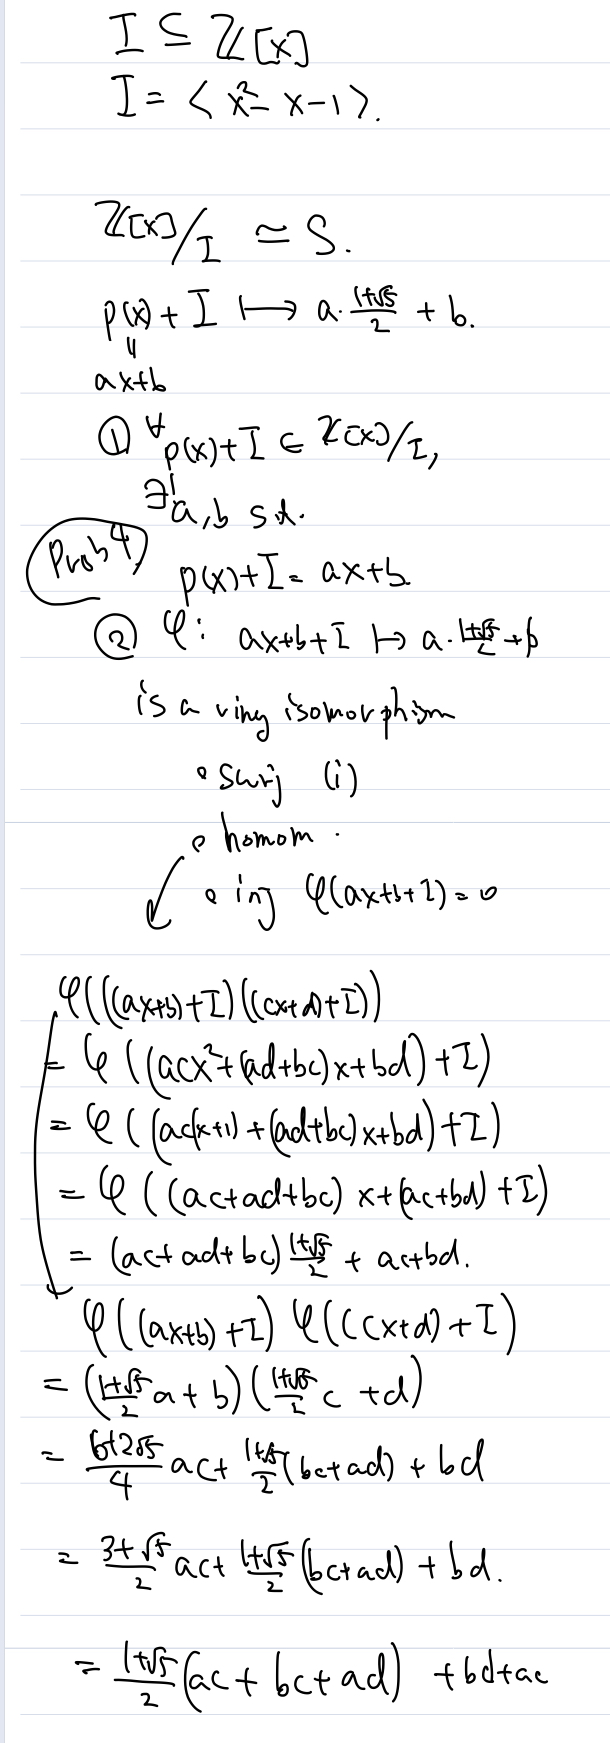
\includegraphics[width=.5\linewidth]{isomorphism.jpeg}
        \caption{mycaption}
        \label{fig:iso}
      \end{figure}
      \begin{itemize}
        \item
          Well-defined?
          By Problem 4, every element in $\mathbb{Z}[x] / I$ can be expressed uniquely as $ax + b + I$ where $a, b \in \mathbb{Z}$.
          (We explicitly used division with remainder to prove Problem 4.)
      \end{itemize}
  \end{enumerate}
\end{proof}

\end{document}


